\begin{figure}
  \centering 
  \begin{subfigure}[b] 
{0.45\textwidth}
    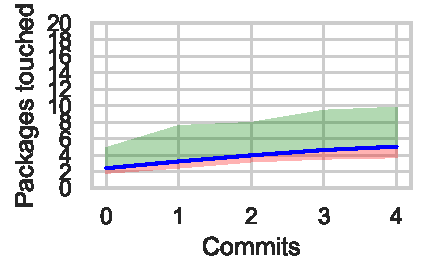
\includegraphics{sections/results/packages/time_series_components_touched.packages.all.founders.commits_5.pdf}
    \caption{Packages for All founders (n=74, $\mu$=5.07, median=3.0 \& std=3.73)}
    \label{figure.sections/results/packages/time_series_components_touched.packages.all.founders.commits_5.pdf}
  \end{subfigure}
  \begin{subfigure}[b] 
{0.45\textwidth}
    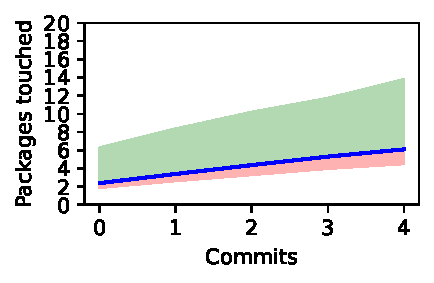
\includegraphics{sections/results/packages/time_series_components_touched.packages.all.joiners.commits_5.pdf}
    \caption{Packages for All joiners (n=783, $\mu$=6.31, median=3.0 \& std=4.82)}
    \label{figure.sections/results/packages/time_series_components_touched.packages.all.joiners.commits_5.pdf}
  \end{subfigure}
\newpage 
\vspace{3mm}
  \begin{subfigure}[b] 
{0.45\textwidth}
    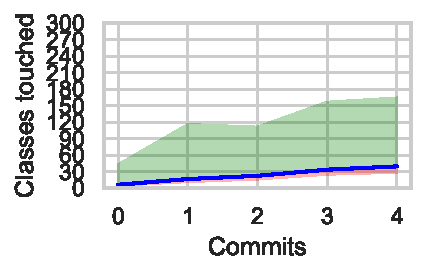
\includegraphics{sections/results/classes/time_series_components_touched.classes.all.founders.commits_5.pdf}
    \caption{Classes for All founders (n=74, $\mu$=39.05, median=7.0 \& std=54.56)}
    \label{figure.sections/results/classes/time_series_components_touched.classes.all.founders.commits_5.pdf}
  \end{subfigure}
  \begin{subfigure}[b] 
{0.45\textwidth}
    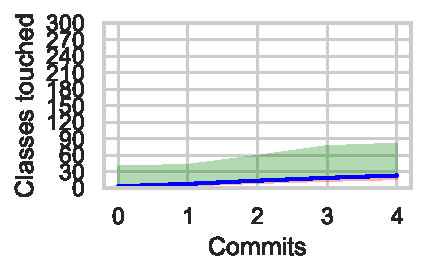
\includegraphics{sections/results/classes/time_series_components_touched.classes.all.joiners.commits_5.pdf}
    \caption{Classes for All joiners (n=783, $\mu$=24.11, median=6.0 \& std=31.7)}
    \label{figure.sections/results/classes/time_series_components_touched.classes.all.joiners.commits_5.pdf}
  \end{subfigure}
\newpage 
\vspace{3mm}
  \begin{subfigure}[b] 
{0.45\textwidth}
    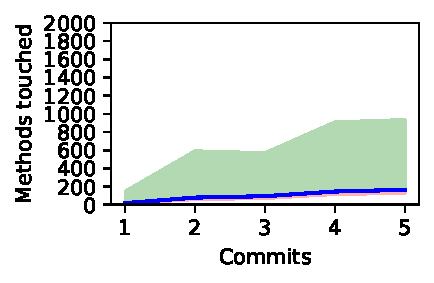
\includegraphics{sections/results/methods/time_series_components_touched.methods.all.founders.commits_5.pdf}
    \caption{Methods for All founders (n=74, $\mu$=164.59, median=20.0 \& std=312.13)}
    \label{figure.sections/results/methods/time_series_components_touched.methods.all.founders.commits_5.pdf}
  \end{subfigure}
  \begin{subfigure}[b] 
{0.45\textwidth}
    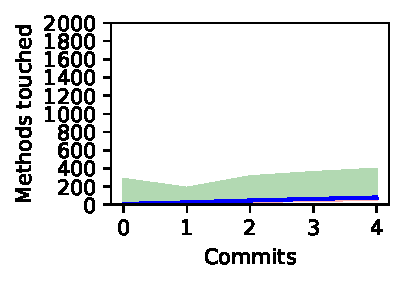
\includegraphics{sections/results/methods/time_series_components_touched.methods.all.joiners.commits_5.pdf}
    \caption{Methods for All joiners (n=783, $\mu$=86.68, median=14.0 \& std=162.09)}
    \label{figure.sections/results/methods/time_series_components_touched.methods.all.joiners.commits_5.pdf}
  \end{subfigure}
\caption{A time series for the five (5) commits, excluding transient, with the average mean (blue line), all components touched (y-axis) against the number of commits (x-axis) for four (4) developer categories. Green is the standard deviation above the mean, and pink is the standard deviation below the mean.}\end{figure}
\clearpage 
\newpage 
